\documentclass{article}
\usepackage[utf8]{inputenc}
\usepackage{graphicx}
\usepackage{mathtools}
\usepackage[export]{adjustbox}
\usepackage[margin=.95in]{geometry}
\setlength\parindent{0pt}
\begin{document}
\title{Unofficial Practice Final Examination}
\makeatletter
\begin{flushright}
\makebox[0.5\textwidth]{Name:\hrulefill}
\end{flushright}
\textbf{Mathematics 263
\newline
\@title}
\newline\newline
\textbf{Instructions:} The unrestricted use of calculators and tables on this examination necessitates requiring that \textbf{all supporting work be shown in order to receive credit}. Experimental work should be performed on the scratch paper provided and will not be graded. The numbered problems are equally weighted in value. Good luck.
\newline\newline
1. (a) Find the angle $\theta$ in Figure 12 Below.
\begin{flushright}
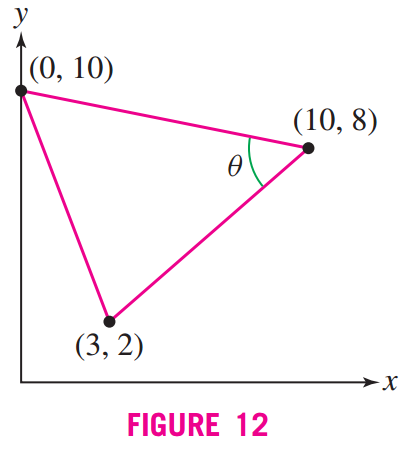
\includegraphics[width=5cm,right]{images/CalcTestPicture3.png}
\end{flushright}
\vfill
(b) Let $\vec{v}= < 4,-1,5>$ and $\vec{v}=< 2,1,1 >$. Find the decomposition $\vec{v}$ = $\vec{v}_{\bot \vec{w}}$ + $\vec{v}_{\perp \vec{w}}$.
\vfill
\vfill

\newpage

\begin{flushleft}
2
\end{flushleft}
2. Find the area enclosed by the cardioid given in polar coordinates by $r = r(\theta) = 1 + \cos (2\theta),$ $0 \leq \theta \leq 2\pi$. Provide a rough sketch to support your work.

\newpage
\begin{flushright}
3
\end{flushright}
3. Evaluate these integrals using any method or combination of methods that we have learned throughout this semester.
\newline \newline
(a) $\displaystyle \int cos^3 \theta $ $ sin^8 \theta $ $d\theta$ Hint: p.440 \#3
\vfill
(b) $\displaystyle \int \frac{dx}{x-x^-1}$ Hint: p.440 \#10
\vfill
(c) $\displaystyle \int \frac{dx}{x^2+4x-5}$  Hint: p.440 \# 12
\vfill

\newpage
\begin{flushleft}
4
\end{flushleft}
4. (a) Classify the following series as \textbf{divergent, absolutely convergent,} or \textbf{conditionally convergent}. Show all work.
$$\sum_{n=1}^{\infty} (-1)^n\frac{n}{n^2+4}$$
\vfill
(b) Classify the following series as \textbf{convergent} or \textbf{divergent}. State which test(s) you are using.
$$\sum_{n=1}^{\infty} (\frac{n}{2n+3})^n$$
\vfill

\newpage
\begin{flushright}
5
\end{flushright}
5. (a) Prove whether the series converges or diverges. If the series converges find the interval of convergence. $$\sum_{n=1}^{\infty} n (x-3)^n$$
\vfill
(b) Find the interval of convergence of the following series. $$\sum_{n=12}^{\infty} e^n (x-2)^n$$
\vfill

\newpage
\begin{flushleft}
6
\end{flushleft}
6. (1) Recall the useful observation that $1+x+x^2+x^3+\dotsi$ is a geometric series, converging to $\displaystyle \frac{1}{1-x}$ on the interval $|x| < 1$. (2) Recall also that $\frac{d}{dx}\tanh^{-1}(x) = \frac{1}{1-x^2}$. Combining these two facts, you can effortlessly find the Maclaurin series for $\frac{d}{dx}\tanh^{-1}(x)$. Do so. Then integrate the resulting series term-by-term to get the Maclaurin series for $f(x) = \tanh^{-1}(x)$. There will be a constant $C$ of integration, it will be useful to know that $\tanh^{-1}(0) = 0$ in order to determine the value of $C$.

\newpage
\begin{flushright}
7
\end{flushright}
7. (a) Find the area of the region that lies inside one but not both of the curves. \textbf{Hint:} pg. 608 \#22
\begin{flushright}
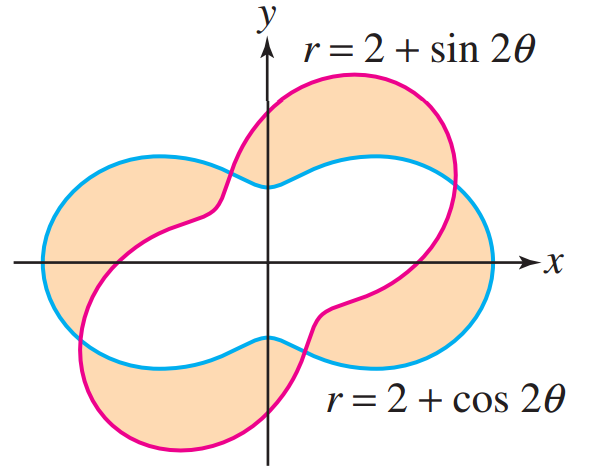
\includegraphics[width=5cm,right]{images/CalcTestPicture4.png}
\end{flushright}
\vfill
(b) Find the area of the shaded region A in the figure below. \textbf{Hint:} pg. 608 \#13
\begin{flushright}
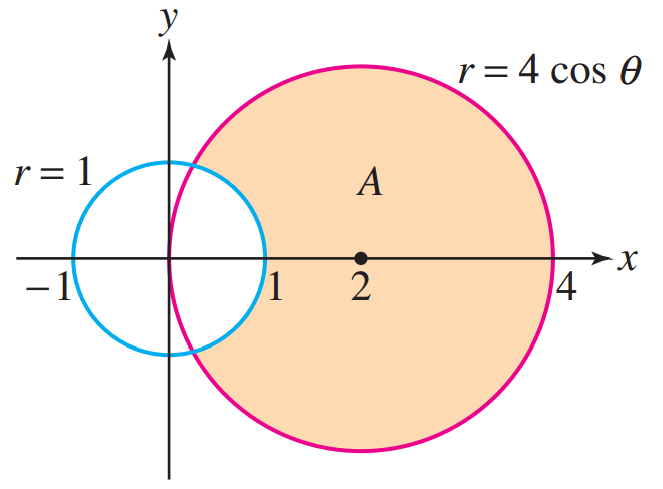
\includegraphics[width=5cm,right]{images/CalcTestPicture5.png}
\end{flushright}
\vfill

\newpage
\begin{flushleft}
8
\end{flushleft}
8. (a) Find the first four non-zero terms of the Taylor series for $f(x) = 4$ $\sqrt[]{x}$ centered at $a = 4$.
\vfill
(b) Find the MacLaurin series for $\displaystyle\frac{1}{1 + 4x^2} + \frac{3}{1-2x^2}$
\vfill

\newpage
\begin{flushright}
9
\end{flushright}
9. (a) Find the Taylor series centered at c and the interval
on which the expansion is valid for $$f(x) = x^4 + 3x - 1, c=2$$
\vfill
(b) Now find the Taylor series centered around $c=0$.
\vfill

\newpage
\begin{flushleft}
10
\end{flushleft}
10. Find the Maclaurin series for the function $f(x) = 2 + 4x + 6x^5 + 8x^9 + 10x^{11}$.
\end{document}
